\section{Evaluation}\label{sec:evaluation}

	All experiments were conducted on a single machine.
	We use macOS 10.14.2 with 8-Core 3.2GHz Intel Xeon W processor, 32 GB DDR4 ECC main memory and 1 TB SSD disk.
	The main code is written in {\Csharp} and runs on {.NET Core 2.1.3}.

	\subsubsection*{Interactive website}\label{sec:website}

		Additionally to making our source code, compiled binaries and Docker images available, we want to let researchers interactively run small-sized simulations.
		We host a website~\cite{ore-website} where one can select a protocol (including baselines, CLOZ and both SSE schemes), cache size and policy and I/O page parameter; supply one's own data and query sets, and run the simulations.
		Simulations are run one at a time and usually complete within seconds.
		The user is then able to view the result --- tables, plots, values and raw JSON, which we used to build plots for this paper.
		Input size on the website is limited for practical purposes and users are encouraged to run arbitrary-size simulations using our binaries or Docker images.

		\begin{table}[t]
	\centering
	\caption{Simulation results for ORE primitive usage}\label{tbl:primitive-usage-result}
	\begin{tabular}{ l c c c }

		\toprule

		Scheme										& Encryption				& Comparison								& Size (bits)			\\

		\toprule

		BCLO~\cite{bclo-ope}					& $\bm{41}$ \textbf{HG}		& none										& $64$					\\

		\midrule

		CLWW~\cite{clww-ore}					& 32 PRF 					& none										& $64$					\\

		\midrule

		\multirow{3}{*}{Lewi-Wu~\cite{lewi-wu-ore}}	& $\bm{32}$ \textbf{PRP}	& \multirow{3}{*}{9 Hash}					& \multirow{3}{*}{2816}	\\
													& 160 PRF					&											&						\\
													& 64 Hash					&											&						\\

		\midrule

		\multirow{3}{*}{CLOZ~\cite{parameter-hiding-ore}}	& 32 PRF					& \multirow{3}{*}{$\bm{1046}$ \textbf{PPH}}	& \multirow{3}{*}{4096}	\\
													& 32 PPH					&											&						\\
													& 1 PRP						&											&						\\

		\midrule

		FH-OPE~\cite{fh-ope}						& 1 Traversal 				& 1 Traversal								& $\bm{86842}$			 \\

		\bottomrule

	\end{tabular}
\end{table}


	\subsection{Implementation}

		We have implemented most of the primitives, data structures, and constructions ourselves.
		For some primitives and all schemes we provided the first open-sourced cross-platform {\Csharp} implementation.
		We note that neither primitives, nor schemes are production-ready; however, we believe they can be used in research projects and prototypes.
		We also emphasize that the {\BPlus} tree implementation we are using, although our own with instrumentation in it, is not custom in any way, but rather standard as defined in the original paper~\cite{b-tree} with deletion algorithm by~\cite{b-plus-tree-deletion}.

		This software project (22K lines of code, third of which are tests) is documented and tested (over 97\% coverage).
		All code including primitives, data structures, schemes, protocols, simulation logic, benchmarks, build scripts and tests is published on GitHub~\cite{ore-project} under CC BY-NC 4.0 license.
		Additionally, we have published parts of the project as stand-alone {.NET Core} (nuGet) packages, and we host a web-server where users can run simulations for small inputs (see previous subsection).

		\subsubsection{Primitives}

			All schemes and protocols use the same primitives, most of which we implemented ourselves.
			All primitives rely on the default {.NET Core} AES implementation.
			{.NET Core} uses platform-specific implementation of AES, thus leverages \texttt{AES-NI} CPU instruction.
			In our project all key sizes are 128 bits, as is AES block size.

			We implemented AES-based PRG, which uses AES in CTR mode and caches unused entropy (as suggested in~\cite{aes-ctr-rfc}).
			For PRF, since we need only 128-bit inputs and outputs, we used one application of AES~\cite[Proposition 3.27]{intro-to-modern-crypto}.
			For symmetric encryption we use AES with a random initialization vector in CBC mode~\cite[Section 3.6.2]{intro-to-modern-crypto}.
			For hash we use default {.NET Core} SHA2 implementation.
			For PRP, we implemented unbalanced Feistel networks~\cite{unbalanced-feistel} for large inputs and Knuth shuffle~\cite{knuth-shuffle} for small inputs.
			Please see the README of project's repository~\cite{ore-project} for low-level details.

		\subsubsection{Schemes and protocols}

			We implemented schemes and protocols precisely as in the original papers.
			When we found problems or improvements, we described them in implementation challenges notes, but did not alter the original designs in our code, unless explicitly stated.
			Each ORE scheme implements a {\Csharp} interface; thus our own implementation of {\BPlus} tree operates on a generic ORE\@.
			For the \emph{no encryption} baseline, we have a stub implementation of the interface, which has identity functions for encryption and decryption.
			It is important to note that all schemes and protocols use exclusively our implementations of primitives.
			Thus we rule out the possible bias of one primitive implementation being faster than the other.

			% \begin{figure}[ht!]
% 	\captionsetup[subfigure]{justification=justified}
% 	\centering
% 	\begin{subfigure}[t]{0.5\linewidth}
% 		\centering
% 		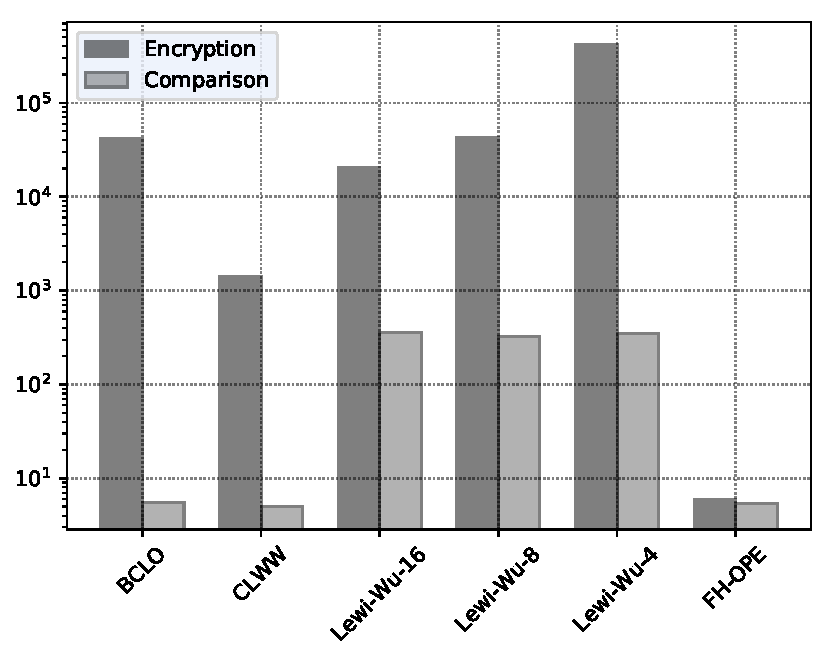
\includegraphics[width=\linewidth]{schemes-benchmark}
% 		\caption{Schemes benchmark (time in microseconds, log scale). Lewi-Wu parameter is the number of blocks.}
% 	\end{subfigure}%
% 	~ % chktex 39
% 	\begin{subfigure}[t]{0.5\linewidth}
% 		\centering
% 		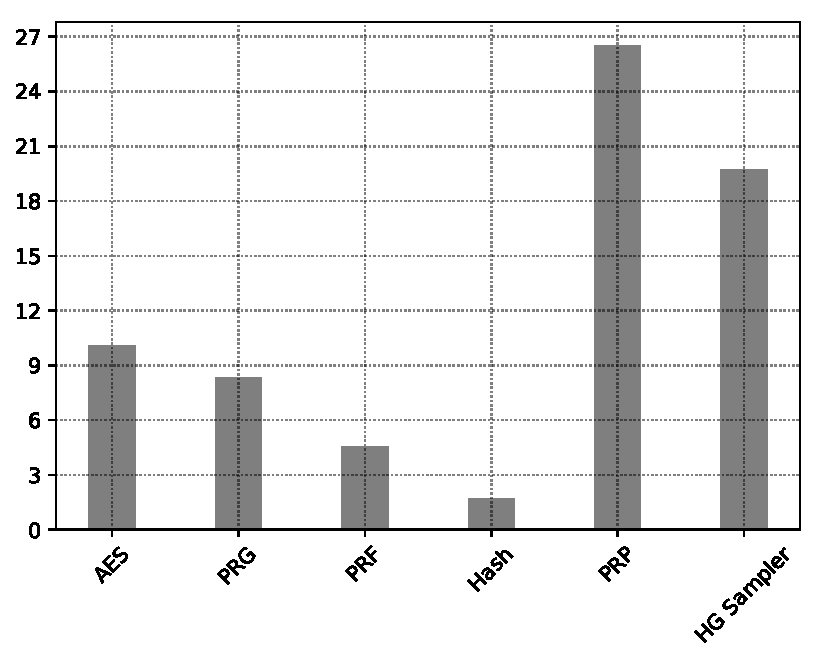
\includegraphics[width=\linewidth]{primitives-benchmark}
% 		\caption{Primitives benchmark (time in microseconds)}
% 	\end{subfigure}%
% 	\caption{Benchmarks of the schemes and primitives}\label{figure:benchmarks}
% \end{figure}

\begin{figure}[!ht]
	\centering
	\begin{minipage}[t]{0.48\columnwidth}
		\centering
		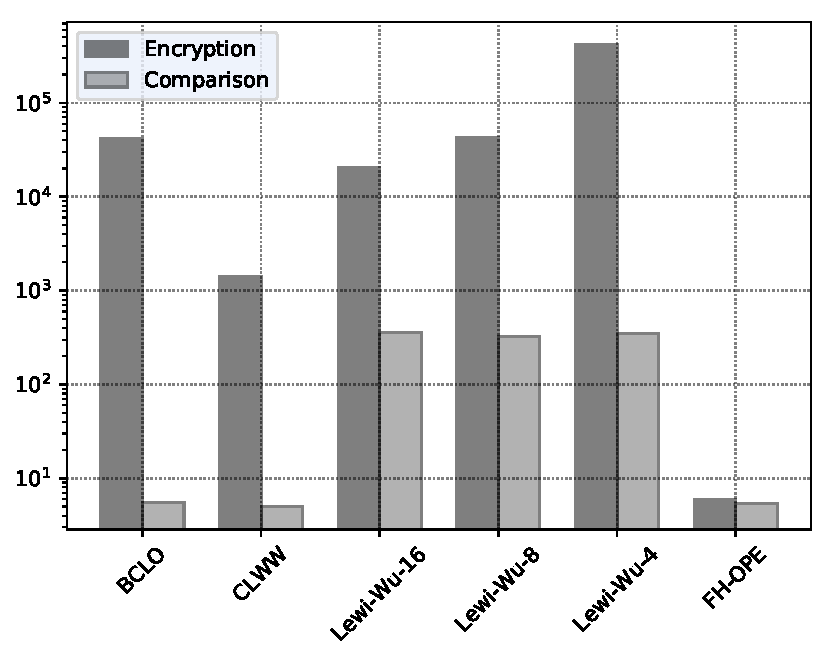
\includegraphics[width=\linewidth]{schemes-benchmark}
		\captionof{figure}{Schemes benchmark (time in microseconds, log scale). Lewi-Wu parameter is the number of blocks.}%
		\label{figure:benchmarks:schemes}
	\end{minipage}
	~ % chktex 39
	\begin{minipage}[t]{0.48\columnwidth}
		\centering
		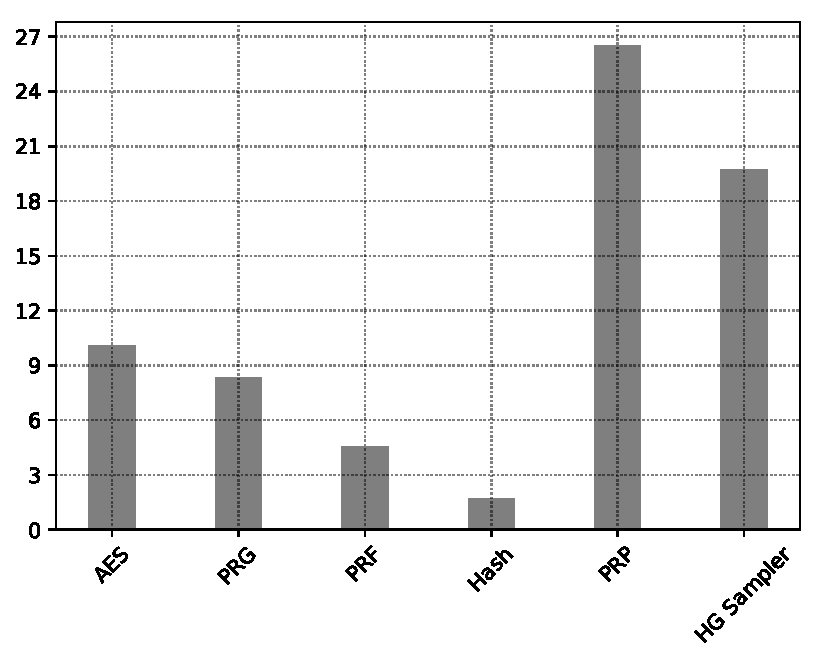
\includegraphics[width=\linewidth]{primitives-benchmark}
		\captionof{figure}{Primitives benchmark (time in microseconds)}%
		\label{figure:benchmarks:primitives}
	\end{minipage}
\end{figure}


		\subsubsection{Simulations}

			\begin{figure*}[ht!]
	\captionsetup[subfigure]{justification=centering}
	\centering
	\begin{subfigure}[t]{0.5\textwidth}
		\centering
		
\includegraphics[width=\linewidth]{protocol-charts-cios}
		\caption{Construction stage number of \acrshort{io} requests}%
		\label{figure:protocols-ios:c}
	\end{subfigure}%
	\hfill
	\begin{subfigure}[t]{0.5\textwidth}
		\centering
		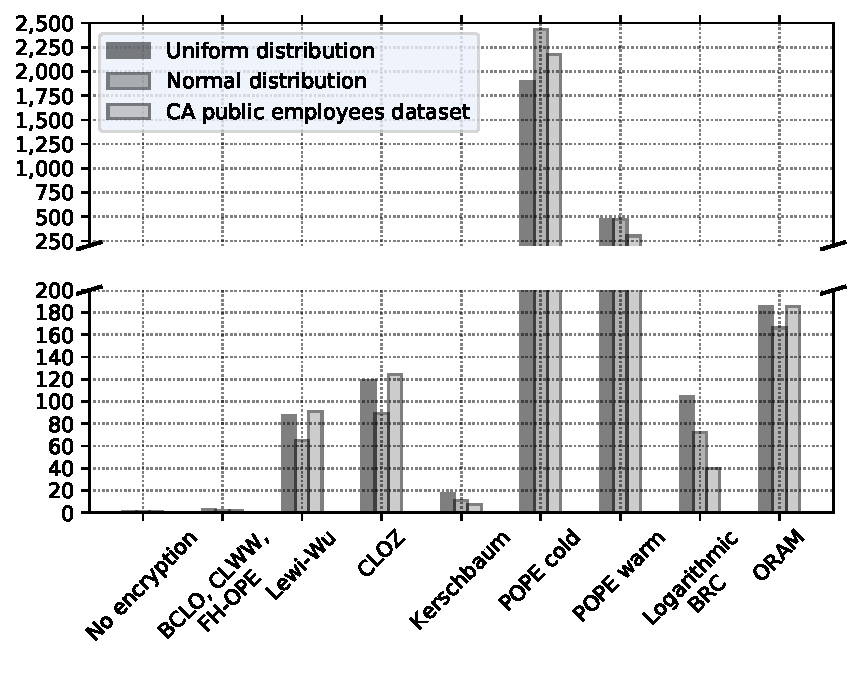
\includegraphics[width=\linewidth]{protocol-charts-qios}
		\caption{Queries stage number of \acrshort{io} requests}%
		\label{figure:protocols-ios:q}
	\end{subfigure}%
	\caption{Number of \acrshort{io} requests for different protocols and data distributions}%
	\label{figure:protocols-ios}
\end{figure*}

\begin{figure*}[ht!]
	\captionsetup[subfigure]{justification=centering}
	\centering
	\begin{subfigure}[t]{0.5\textwidth}
		\centering
		
\includegraphics[width=\linewidth]{protocol-charts-csize}
		\caption{Construction stage communication size (bytes transferred)}%
		\label{figure:protocols-size:c}
	\end{subfigure}%
	\hfill
	\begin{subfigure}[t]{0.5\textwidth}
		\centering
		
\includegraphics[width=\linewidth]{protocol-charts-qsize}
		\caption{Queries stage communication size (transferred bytes, log scale)}%
		\label{figure:protocols-size:q}
	\end{subfigure}%
	\caption{Communication size for different protocols and data distributions}%
	\label{figure:protocols-size}
\end{figure*}

\begin{figure*}[ht!]
	\captionsetup[subfigure]{justification=centering}
	\centering
	\begin{subfigure}[t]{0.5\textwidth}
		\centering
		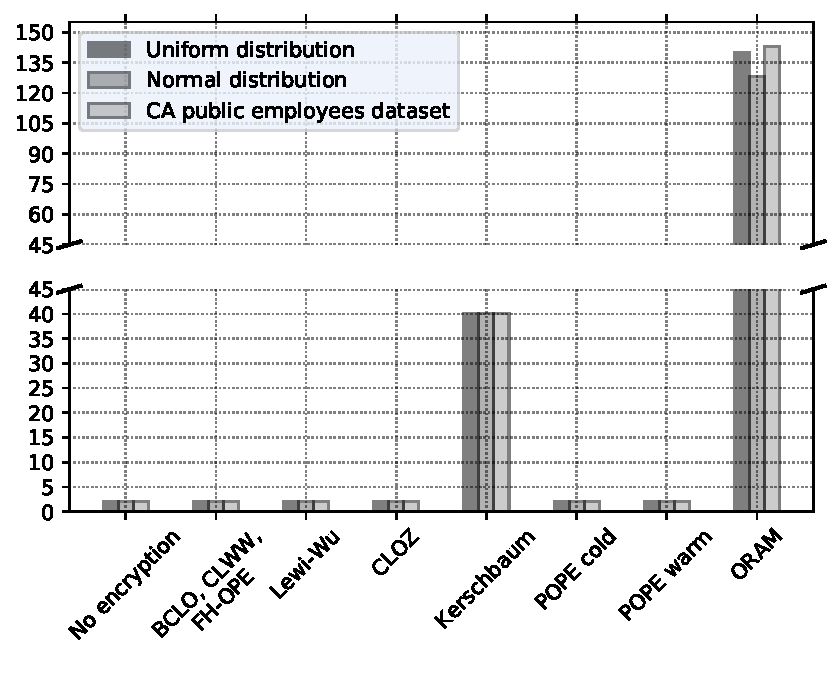
\includegraphics[width=\linewidth]{protocol-charts-cvol}
		\caption{Construction stage communication volume (number of messages)}%
		\label{figure:protocols-vol:c}
	\end{subfigure}%
	\hfill
	\begin{subfigure}[t]{0.5\textwidth}
		\centering
		
\includegraphics[width=\linewidth]{protocol-charts-qvol}
		\caption{Queries stage communication volume (number of messages)}%
		\label{figure:protocols-vol:q}
	\end{subfigure}%
	\caption{Communication volume for different protocols and data distributions}%
	\label{figure:protocols-vol}
\end{figure*}


			We have four types of simulations.

			Protocol simulation runs both protocol stages --- construction and search --- on supplied data for all protocols including all schemes coupled with {\BPlus} tree.
			In this simulation we measure the primitive usage, number of ORE scheme operations (when applies), communication volume and size, and the number of {\IO} requests.
			We intentionally do not measure elapsed time, since it would be extremely inaccurate in this setting --- simulation and measurement routines take substantial fraction of time.

			Scheme simulation runs all five ORE schemes and tracks only the primitive usage.

			The scheme benchmark, however, is designed to track time.
			We use Benchmark.NET~\cite{benchmark-net} to ensure that the reported time is accurate.
			This tool handles issues like cold / warm start, elevating process' priority, and performing enough runs to draw statistically sound conclusions.
			This benchmark reports elapsed time up to nanoseconds for all four schemes (excluding CLOZ) and their variants.

			Finally, primitive benchmark uses the same tool, but compares the primitives.
			We use it to compare different implementations of primitives (e.g.\ Feistel PRP vs pre-generated permutation) and to approximate time consumption of the schemes and protocols based on primitive usage.

	\subsection{Setup}

		For our simulations, we have used three datasets.
		Two synthetic distributions, that are uniform (range is third of data size) and normal (standard deviation is $0.1$ of data size).
		The real dataset is California public employees salaries (``total pay and benefits'' column)~\cite{ca-dataset}.
		Synthetic datasets and subsets of the real dataset are generated pseudo\hyp{}randomly.
		Queries are generated uniformly at random with a range as a percentage of data size.

	\subsection{Results}

		\subsubsection{Primitive usage by schemes}\label{sec:schemes-primitive-usage}

			In Table~\ref{tbl:primitive-usage-result} we show the simulation-derived values of each OPE and ORE scheme's primitive usage.
			Each scheme is given 1000 data points of each dataset.
			First, the scheme encrypts each data point, then decrypts each ciphertext and then performs five comparisons (all possible types) pairwise.
			This micro-simulation is repeated 100 times.
			Resulting values for primitive usage are averaged for each scheme.
			State and ciphertext sizes are calculated after each operation and the values are averaged.
			Please note that the simulated values are consistent with the theoretical calculations.

		\subsubsection{Benchmarks of schemes and primitives}

			Using the Benchmark.NET tool~\cite{benchmark-net}, we have accurately tracked the performance of the schemes and primitives running of different parameters (see Figure~\ref{fig:benchmarks}).
			ORE schemes benchmark setup is the same as in primitive usage simulation~\ref{sec:schemes-primitive-usage}.
			Primitives were given randomly generated byte inputs and keys of different sizes (e.g.\ PRP of $2$ to $32$ bits).
			Benchmark.NET decides how many times to run the routine to get statistically sound results.
			For example, large variance results in more runs.
			To improve the accuracy, each run is compiled in release mode as a separate project and runs in a separate process with the highest priority.

			Please note the logarithmic scale of the schemes' performances.
			FH-OPE is fast since it does not perform CPU-heavy operations and works in main memory.
			Lewi-Wu performance degrades exponentially with the increase of block size mainly due to exponential number of PRF executions and the performance of PRP degrading exponentially.
			Note also that Lewi-Wu comparison takes noticeable time due to Hash primitive usage.

			In the primitives benchmark, it is clear that most primitives use AES under the hood.
			PRG and PRF take less than AES because they do not include the initialization vector generation needed for symmetric encryption.
			PRP is implemented as a Knuth shuffle~\cite{knuth-shuffle} and its complexity is exponential in the input bit length.
			Input size of 2 bits is shown on Figure~\ref{fig:benchmarks}.
			PRG does not discard the entropy generated by AES cycle, so one AES cycle can supply four 32-bit integers.
			PRP generates the permutation table once and does not regenerate it if the same key and number of bits are supplied.

		\subsubsection{Protocols}\label{sec:results-protocols}

			In this experiment we have run each protocol with each of the three datasets.
			Dataset sizes are 247000 (bounded by California Employees dataset size) and the number of queries is 1000.
			Queries are generated uniformly at random with a fixed range --- 0.5\% of data size.
			The cache size is fixed to 128 blocks, and the {\BPlus} tree branching factor as well as block sizes for other protocols are set such that the page size is 4 kilobytes.
			The values we are measuring are the number of {\IO} operations, communication volume, and size for both construction and query stages.

			See Table~\ref{tbl:protocols-result} for the snapshot for particular distribution (CA employees).
			Figure~\ref{fig:protocols} shows all values we tracked for all protocols and distributions.
			Values for ORE based protocols are averaged.
			Being ``cold'' in our simulations means executing the first query and being ``warm'' means the first query has been previously executed.
			This difference makes sense only for POPE as its first query incurs disproportionately large overhead by design.

			Note that all ORE based protocols behave the same except when ciphertext size matters.
			Thus, since BCLO, CLWW and FH-OPE have the same ciphertext size, they create {\BPlus} trees with the same page capacity and have the same number of {\IO}s for different operations.
			Lewi-Wu and CLOZ schemes have relatively large ciphertexts and thus induce larger traffic (see Subfigure~\ref{fig:protocols:csize}) and smaller {\BPlus} tree branching factor resulting in greater number of {\IO} requests (see Subfigure~\ref{fig:protocols:qios}).
			Kerschbaum protocol requires high number of {\IO} requests during construction since it needs to insert an element into the arbitrary place in an array and rotate the data structure on a disk.

			POPE suffers huge penalty on the first query (see Subfigures~\ref{fig:protocols:qios},~\ref{fig:protocols:qvol} and~\ref{fig:protocols:qsize}) since it reads and sends all blocks to the client for sorting.
			POPE performance improves as more queries are executed.

			Logarithmic\hyp{}BRC does not support interactive insertions and thus its construction stage is not benchmarked.
			Otherwise it is the most performant of all non-ORE protocols.
			Note, however, that its performance depends on the result size, not data size.

			As expected, ORAM performs worse than the ORE-based protocols, but its performance is in-line with the non-ORE protocols.
			It may seem that ORAM does especially bad in construction communication (Subfigures~\ref{fig:protocols:qvol},~\ref{fig:protocols:qsize}), but it is only because POPE has a shortcut in construction.
			This ``debt'' is being payed off during queries (Subfigure~\ref{fig:protocols:qsize}).

			Note that the values do not vary a lot among different data distributions except for {\IO} requests.
			{\IO} performance depends on the result size for queries, and is therefore more sensitive to data distribution.

			Also note that using an ORE scheme with relatively small ciphertext in {\BPlus} tree does not add any substantial {\IO} overhead (see ``No encryption'').

			On Figure~\ref{fig:protocols-query-sizes} it is clear that query performance does not depend substantially on the query size, except for Logarithmic\hyp{}BRC, for which the relation is linear.
			Note that Logarithmic\hyp{}BRC with optimally configured \texttt{pack} extension shows almost no growth.
			This is because for large ranges BRC will return the higher nodes (keywords matching many documents), which are optimally packed in {\IO} pages.
			As query range doubles, higher nodes are involved increasing the chance that requested keywords have their documents packed.

			\newlength{\hardcodedheighto}
\newlength{\askipo}
\newlength{\bskipo}
\newlength{\blskipo}

\setlength{\hardcodedheighto}{135pt}
\setlength{\askipo}{-10pt}
\setlength{\bskipo}{0pt}
\setlength{\blskipo}{-5pt}

\begin{figure*}[ht!]	
	\captionsetup{justification=centering}
	\centering
	\begin{minipage}{0.66\textwidth}
		\captionsetup[subfigure]{justification=centering}
		\centering
		\begin{subfigure}[t]{0.5\textwidth}
			\centering
			
\includegraphics[height=\hardcodedheighto,width=\linewidth]{protocol-data-percent-cios.pdf}
			\setlength{\abovecaptionskip}{\askipo}
			\setlength{\belowcaptionskip}{\bskipo}
			\caption{Construction stage {\IO} requests}\label{fig:protocols-data-percent:cios}
		\end{subfigure}%
		~ % chktex 39
		\begin{subfigure}[t]{0.5\textwidth}
			\centering
			
\includegraphics[height=\hardcodedheighto,width=\linewidth]{protocol-data-percent-cvol.pdf}
			\setlength{\abovecaptionskip}{\askipo}
			\setlength{\belowcaptionskip}{\bskipo}
			\caption{Construction stage number of messages}\label{fig:protocols-data-percent:cvol}
		\end{subfigure}%
	
		\begin{subfigure}[t]{0.5\textwidth}
			\centering
			
\includegraphics[height=\hardcodedheighto,width=\linewidth]{protocol-data-percent-qios.pdf}
			\setlength{\abovecaptionskip}{\askipo}
			\setlength{\belowcaptionskip}{\blskipo}
			\caption{Queries stage {\IO} requests}\label{fig:protocols-data-percent:qios}
		\end{subfigure}%
		~ % chktex 39
		\begin{subfigure}[t]{0.5\textwidth}
			\centering
			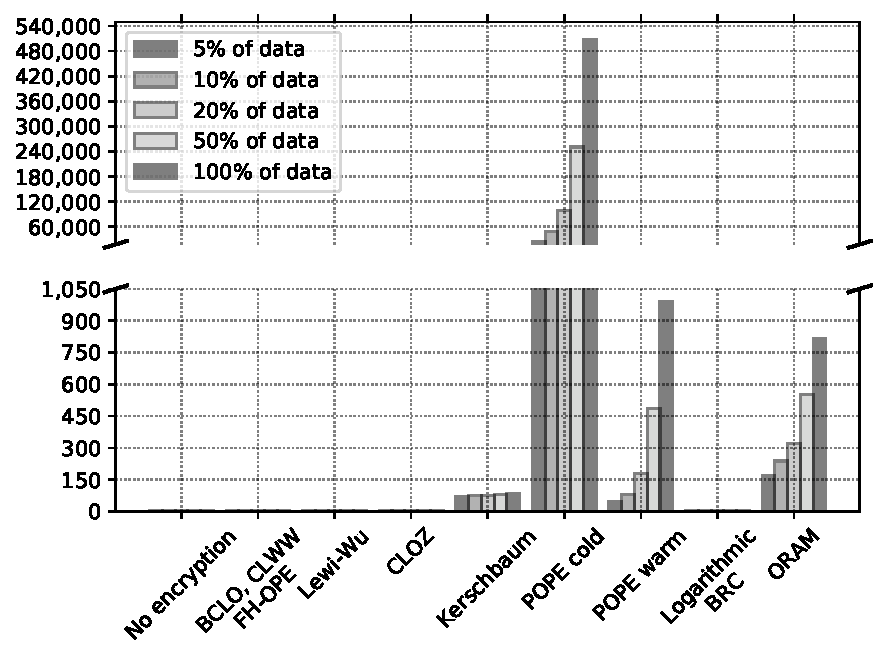
\includegraphics[height=\hardcodedheighto,width=\linewidth]{protocol-data-percent-qvol.pdf}
			\setlength{\abovecaptionskip}{\askipo}
			\setlength{\belowcaptionskip}{\blskipo}
			\caption{Queries stage number of messages}\label{fig:protocols-data-percent:qvol}
		\end{subfigure}%
		\caption{Protocol scalability}\label{fig:protocols-data-percent}
	\end{minipage}%
	\begin{minipage}{.33\textwidth}
		\captionsetup[subfigure]{justification=centering}
		\centering
		\begin{subfigure}[t]{\textwidth}
			\centering
			\setlength{\abovecaptionskip}{-0pt}
			\setlength{\belowcaptionskip}{\bskipo}
			
\includegraphics[height=\hardcodedheighto,width=\linewidth]{protocol-query-sizes-ios.pdf}
			\caption{For different query sizes}\label{fig:protocols-query-sizes}
		\end{subfigure}%

		\begin{subfigure}[t]{\textwidth}
			\centering
			
\includegraphics[height=\hardcodedheighto,width=\linewidth]{cold-vs-warm-ios.pdf}
			\setlength{\abovecaptionskip}{\askipo}
			\setlength{\belowcaptionskip}{\blskipo}
			\caption{Over time (queries).}\label{fig:cold-vs-warm}
		\end{subfigure}%
		\caption{Number of {\IO} requests}\label{fig:protocols-different-queries}
	\end{minipage}
\end{figure*}


			Figure~\ref{fig:protocols-data-percent} shows Table~\ref{tbl:protocols} asymptotic values.
			The simulation was run for uniform dataset of 247000 records (hundred percent), 1000 queries, 0.5\% query range and 128 blocks cache size.
			Kerschbaum construction {\IO}s and cold POPE query values grow linearly with inputs, while the other protocols grow logarithmically, square-logarithmically, or do not grow.

			Figure~\ref{fig:cold-vs-warm} shows how the performance of protocols fluctuates as queries are processed.
			Note that POPE and Logarithmic\hyp{}BRC fluctuate the most (which is, in general, undesirable), and POPE is the only protocol where cold versus warm makes a difference.
